\chapter{Numerical simulations}\label{sec:simul}

In this chapter we conduct some experiments to test our safe method. We compare the different variants of our algorithm to observe their performance in practice. We also compare our method with older or more common approaches to see how much the theoretical improvements obtained in the previous chapter translate into better practical results.
In Section \ref{sec:lqg1d} we use a simple simulated control task, one-dimensional \ac{LQG}, to compare the different variants of our algorithm.
In Section \ref{sec:lqg2d} we use a two-dimensional variant of the same problem to show the advantages of our method over older approaches. 

\section{One-Dimensional LQG}\label{sec:lqg1d}
In this section we test the proposed methods on the one-dimensional \ac{LQG} problem \cite{4867}. We use this task as a testing ground because it is simple, all the constants involved in our bounds can be computed exactly, and the optimal parameter $\theta^*$ is available as a reference.

The LQG problem is a continuous \ac{MDP} defined by transition model:
\[
	s_t \sim \mathcal{N}(s_t+a_t,\sigma_0^2),
\] 

reward function:
\[
	r_t=-0.5(s_t^2+a_t^2),
\]
and Gaussian policy:
\[
	a_t \sim \mathcal{N}(\theta\cdot s_t,\sigma^2).
\]
Intuitively, the problem is to bring to zero a system's state, in the presence of noise, with a cost for acting on the system.
The policy has a single parameter $\theta$. The optimal value $\theta^*$ can be computed exactly, but the problem can be used as a benchmark for \ac{RL} algorithms.

In all our simulations we use $\sigma_0 = 0$, since all the noise can be modeled on the agent's side without loss of generality. Both action and state variables are bounded to the interval $[-2,2]$ and the initial state is drawn uniformly at random.  
We use a discount factor $\gamma=0.9$, which gives as optimal parameter $\theta^* \approx -0.59$, corresponding to expected performance $J(\theta^*) \approx -13.21$. The expected performance is very pessimistic, since it doesn't take into account the bound on actions and states and the limited length of the task horizon, but equally captures the progress of the real performance. A monotonically improving expected performance is a guarantee that the policy is improving without oscillation, even if the measured performance is noisy due to stochasticity in the environment and in the policy itself.
\paragraph{}
In our experiments, we are interested both in the convergence speed and in policy oscillation. We call \textit{improvement ratio} the ratio of policy updates that does not result in a worsening of the expected performance. First of all, we want to analyze how the choice of fixed step sizes and batch sizes may affect the improvement ratio and how much it depends on the variability of the trajectories (that in this case is due to the variance of the policy $\sigma$).
Table \ref{tab:1} shows the improvement ratio for two parameterizations ($\sigma=0.5$ and $\sigma=1$) when various constant step sizes and batch sizes are used, starting from $\theta=-0.55$ and stopping after a total of one million trajectories. 

\begin{table}[H]
\caption[Improvement ratio of the policy updates for different parametrizations of the LQG task.]{Improvement ratio of the policy updates for different policy standard deviation $\sigma$, fixed batch size $N$ and fixed step size $\alpha$, using the G(PO)MDP gradient estimator.}
\label{tab:1}
\centering
\begin{adjustbox}{right}
\begin{tabular}{@{}llccccccc@{}} 
\toprule
\phantom{abc} & \phantom{abc} & \multicolumn{3}{c}{$\sigma=0.5$} & \phantom{abc} & \multicolumn{3}{c}{$\sigma=1$} \\
\cmidrule{3-5} \cmidrule{7-9}
\phantom{abc} & \phantom{abc} & $N=10000$ & $N=1000$ & $N=100$ & \phantom{abc} & $N=10000$ & $N=1000$ & $N=100$
\\\cmidrule{3-9}
\phantom{abc} & 1e-3 & 95.96\% & 52.85\% & 49.79\% & \phantom{abc} & 24.24\% & 37.4\% & 50.4\% \\ 
 $\alpha$	  & 1e-4 & 100\% & 73.27\% & 51.41\% & \phantom{abc} & 100\% & 27.03\% & 46.08\% \\
\phantom{abc} & 1e-5 & 98.99\% & 81.88\% & 55.69\% & \phantom{abc} & 100\% & 99.9\% & 39.04\%\\
\phantom{abc} & 1e-6 & 100\% & 83.88\% & 58.44\% & \phantom{abc} & 100\% & 100\% & 86.04\% \\
\bottomrule
\end{tabular}
\end{adjustbox}
\end{table}

As expected, small batch sizes combined with large step sizes lead to low improvement ratios. However, the effect of the meta-parameters is non-trivial and problem-dependent, justifying the need for an adaptive method.  
\paragraph{}
We now proceed to test the methods described in Chapter \ref{chap:main}. 
In all the following simulations we use $\sigma = 1$ and start from $\theta=0$, stopping after a total of 30 million trajectories.

We start by testing Algorithm \ref{alg:adabatch} with Chebyshev's bound as proposed in Section \ref{sec:chebyshev}. To estimate the gradient, we use the REINFORCE and G(PO)MDP gradient estimators. In both cases, we use optimal baseline from \cite{4867}.
Figure \ref{fig:1} shows the expected performance over sample trajectories for the two gradient estimators and for different values of $\delta$, the probability with which worsening updates are allowed to take place.

 To make this and the following figures more interpretable, some words must be spent on how data were processed. Each learning iteration corresponds to a single value of $\theta$, with a corresponding expected performance. The latter was scaled over time, simply by maintaining the value for all the trajectories of the batch (a closer look to the plot would reveal a series of steps of variable length and height). The horizontal scaling was performed to better capture the improvement of performance over time.


\begin{figure}[h!]
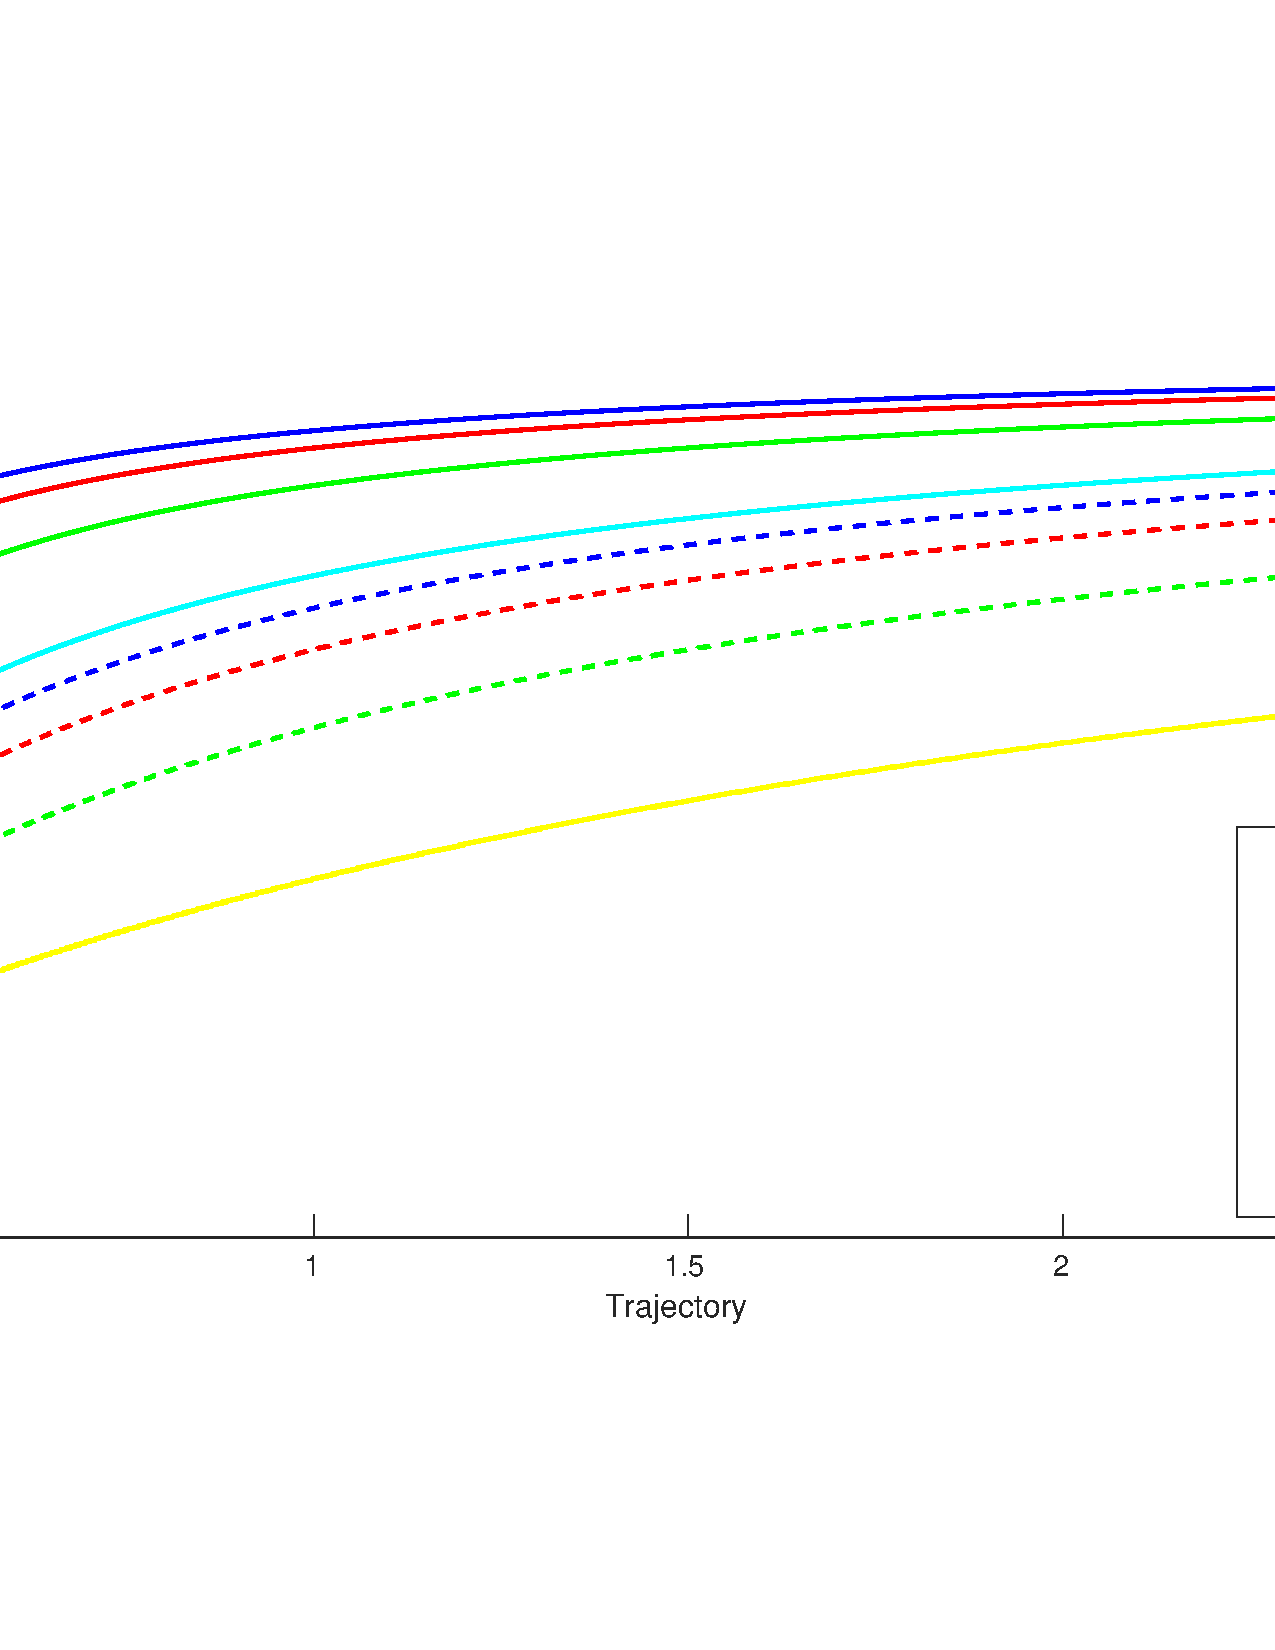
\includegraphics[width = \textwidth,center]{Images/chebyshev.pdf}
\caption[Expected performance over sample trajectories in the one-dimensional LQG task for different gradient estimators ad values of $\delta$.]{Expected performance over sample trajectories in the one-dimensional \ac{LQG} task, using G(PO)MDP and REINFORCE (dashed) gradient estimators and Chebyshev bound, for different values of $\delta$. Expected performance is computed for each parameter update. Data are then scaled to account for the different batch sizes. All results are averaged over 5 runs of 30 million total trajectories each.}
\label{fig:1}
\end{figure}

In general REINFORCE performs worse than G(PO)MDP due to its larger variance.
Larger values of $\delta$  lead to better performance. Notice that an improvement ratio of $1$ is achieved also with large values of $\delta$. This is due to the fact that the bounds used in the development of our method are not tight. Being the method this conservative, in practical applications $\delta$ can be set to a high value to improve the convergence rate.
\paragraph{}
The next step is to compare the Chebyshev's bound approach to the other methods proposed in Section \ref{sec:batchsize}. We stick to the configuration that performed the best in the previous experiment: G(PO)MDP to estimate the gradient and $\delta=0.95$. 
Figure \ref{fig:2} compares the performance of the different concentration bounds.

\begin{figure}[h!]
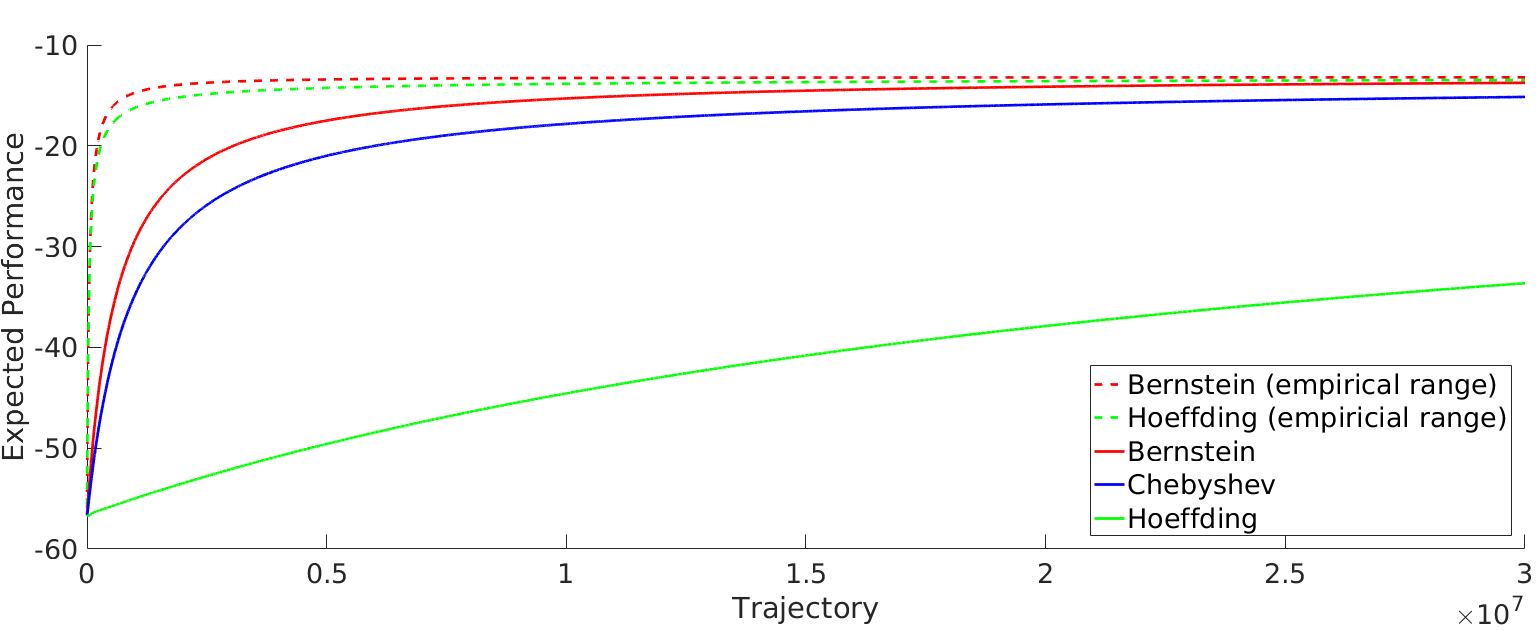
\includegraphics[width = 1.36\textwidth,left]{Images/compare_bounds.png}
\caption[Comparison of the performance of different statistical bounds in the one-dimensional LQG task.]{Comparison of the performance of different statistical bounds in the one-dimensional \ac{LQG} task, using the G(PO)MDP gradient estimator and $\delta=0.95$. All results are averaged over 5 runs.}
\label{fig:2}
\end{figure}

As expected, Bernstein's bound performs better than Chebyshev's, especially in the empirical range version. The rigorous version of Hoeffding's bound performs very poorly, while the one using the empirical range is almost as good as the corresponding Bernstein method. This is due to the fact that the bound on the gradient estimate range is very loose, since it accounts also for unrealistic combinations of state, action and reward.
\paragraph{}
To better capture the performance of the different variants of the algorithm in a real-time scenario, we define a metric $\overline{\Upsilon}$, which is obtained by averaging the real performance (measured during learning) over all the trajectories, coherently with the cost function used to derive the optimal batch size. The results are reported in Table \ref{tab:2}.

\begin{table}[H]
\caption[Average performance in the one-dimensional LQG task for different gradient estimators, statistical bounds and values of $\delta$.]{Average performance in the one-dimensional \ac{LQG} task for different gradient estimators, statistical bounds and values of $\delta$. All results are averaged over 5 runs ($5\%$ confidence intervals are reported).}
\label{tab:2}
\centering
\begin{adjustbox}{right}
\begin{tabular}{llccc}
\toprule
Estimator & Bound &$\delta$ & $\overline{\Upsilon}$ & Confidence interval \\\midrule 
\csvreader[head to column names]{Data/lqg_performance.csv}{}
{\\\csvcoli&\csvcolii&\csvcoliii&\csvcoliv&\csvcolv}
\\\bottomrule
\end{tabular}
\end{adjustbox}
\end{table}

Finally, it is interesting to look at the trend of the batch size over learning iterations. Figure \ref{fig:8} shows the batch size for the different concentration bounds.

\begin{figure}[h!]
\begin{adjustbox}{left}
	\subfloat[Chebyshev]{
	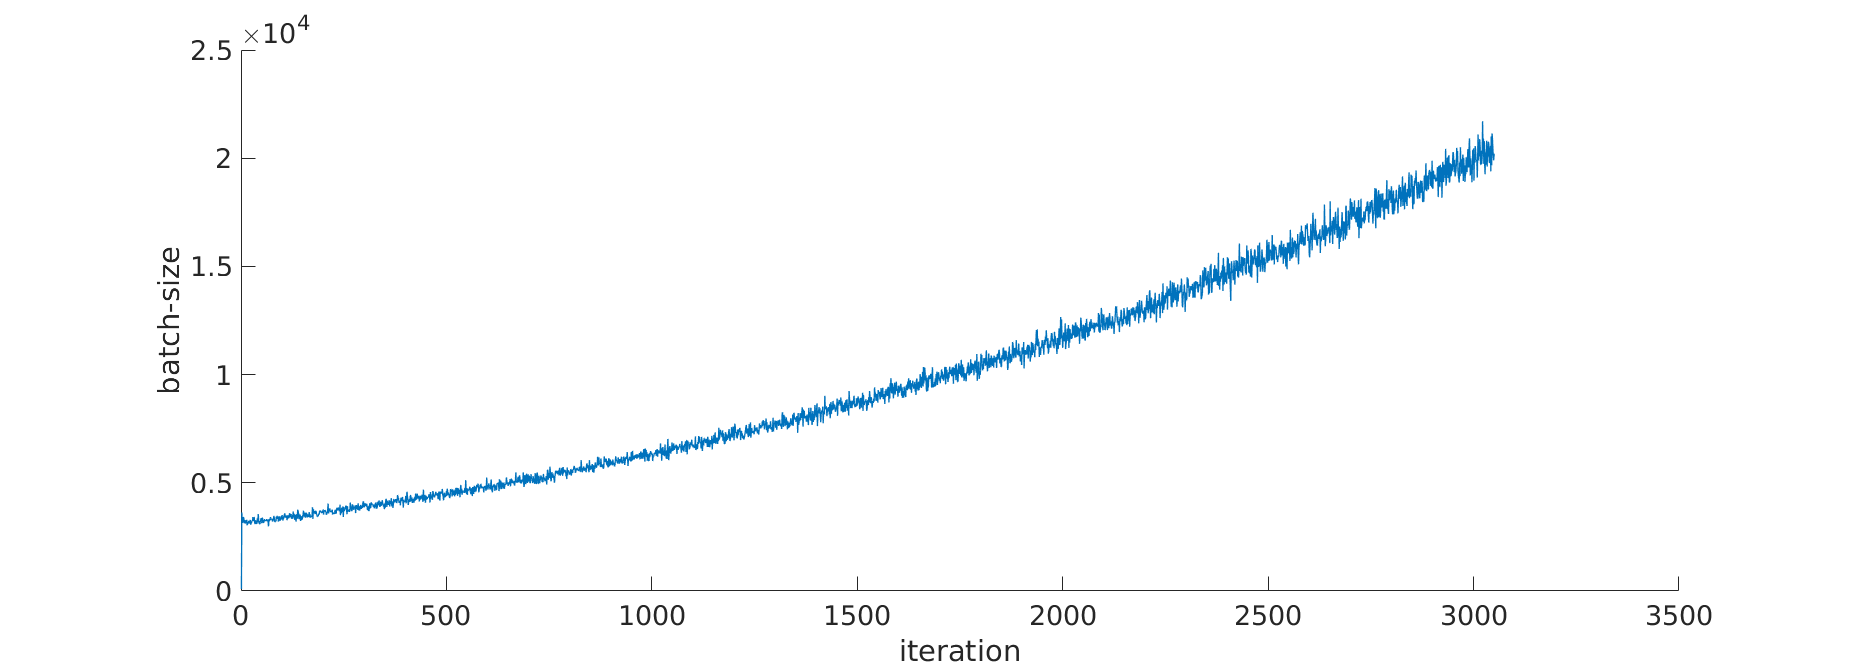
\includegraphics[width = 1.4\linewidth]{Images/batchsize_cheb.png}
	\label{fig:3}
	}
\end{adjustbox}
\begin{adjustbox}{left}
	\subfloat[Hoeffding]{
	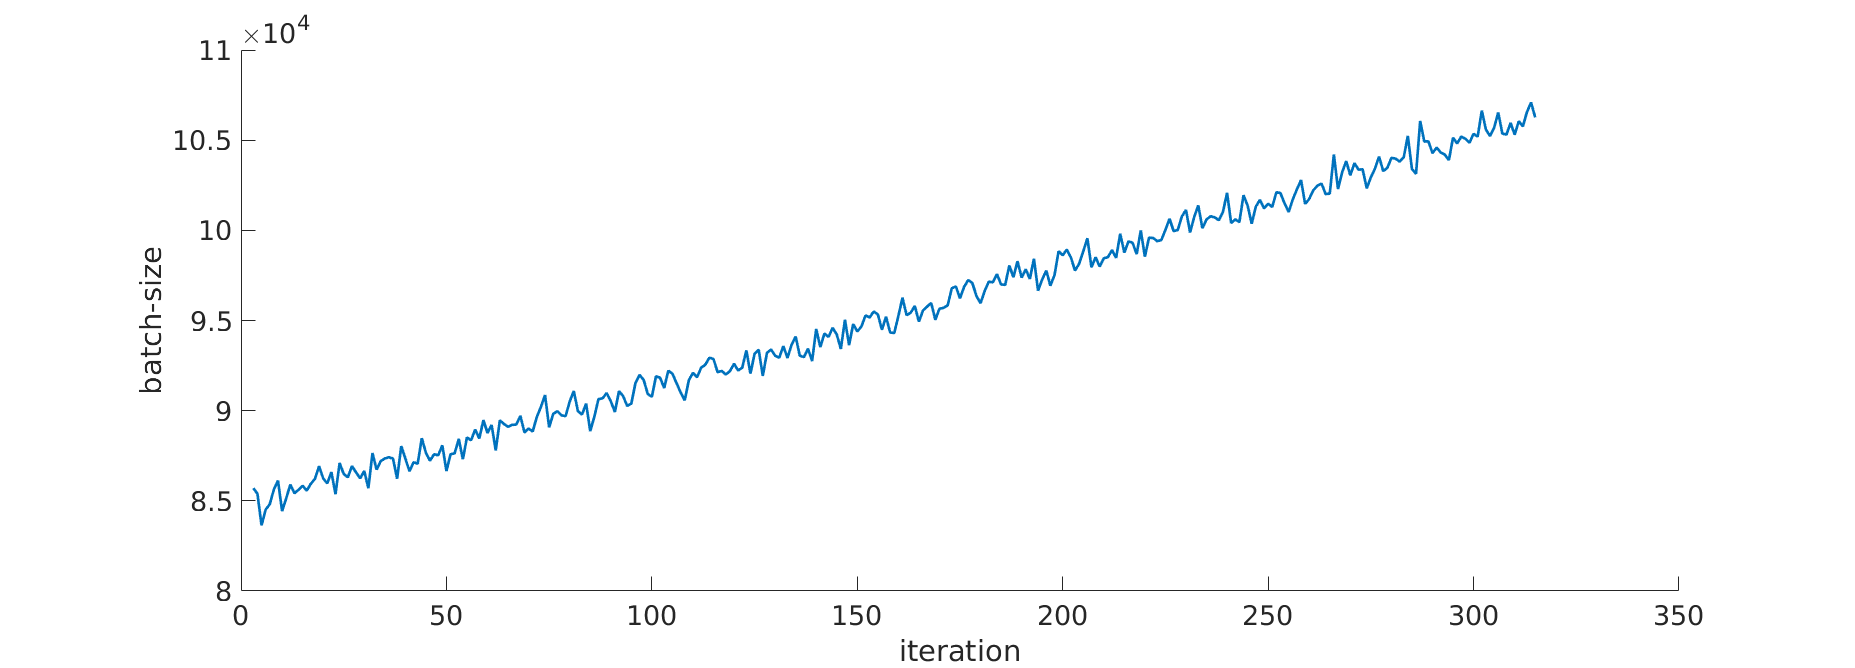
\includegraphics[width = 0.7\linewidth]{Images/batchsize_hoeff.png}
	\label{fig:4}
	}
	\subfloat[Hoeffding with empirical range]{
	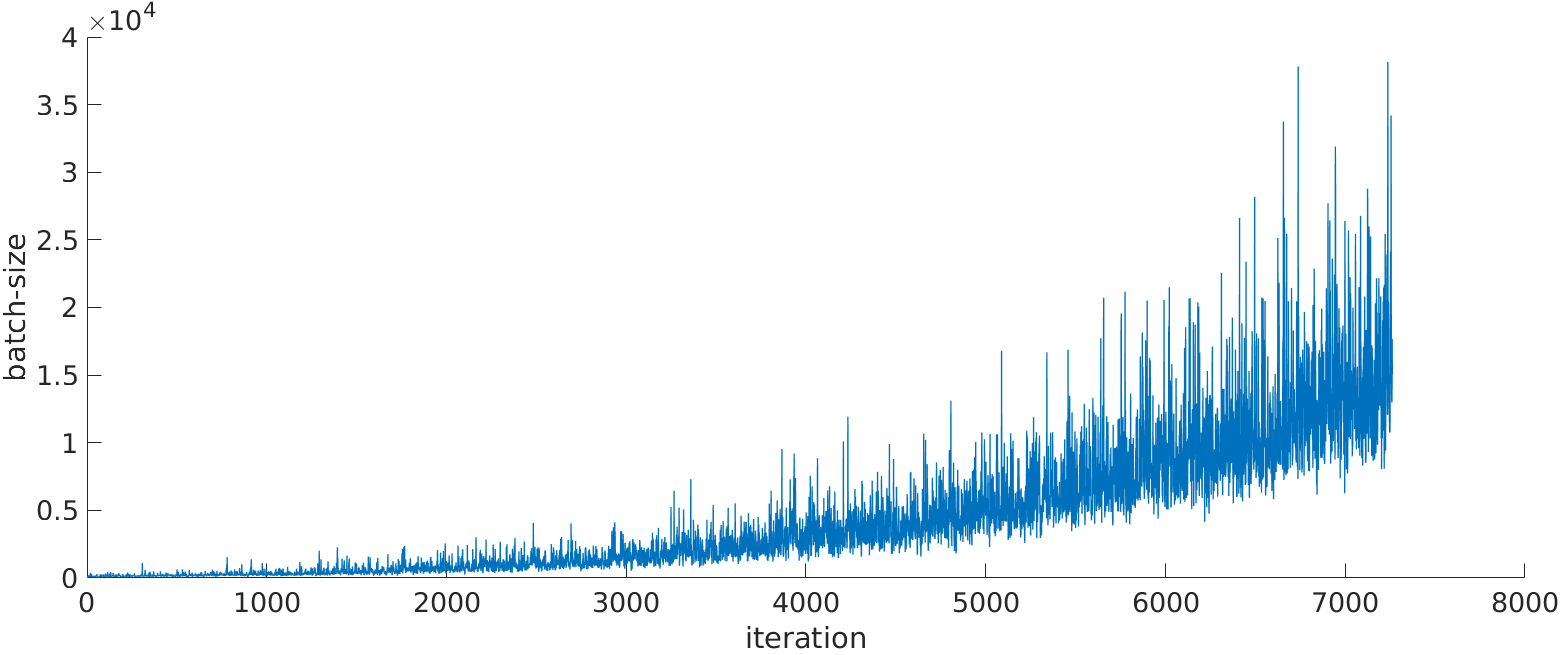
\includegraphics[width = 0.7\linewidth]{Images/batchsize_hoeff_emp.png}
	\label{fig:5}
	}
\end{adjustbox}
\begin{adjustbox}{left}
	\subfloat[Bernstein]{
	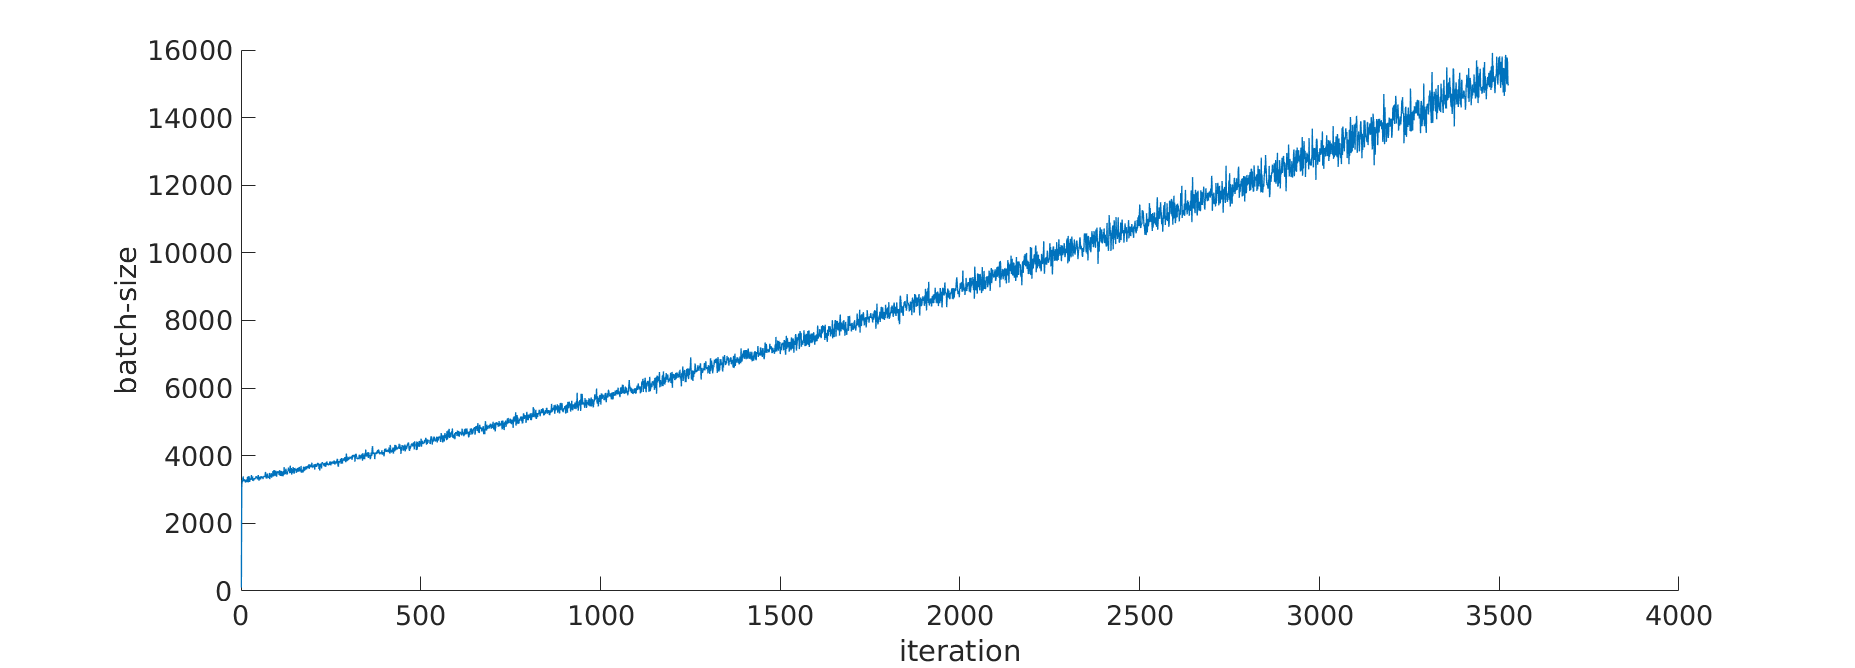
\includegraphics[width = 0.7\linewidth]{Images/batchsize_bern.png}
	\label{fig:6}
	}
	\subfloat[Bernstein with empirical range]{
	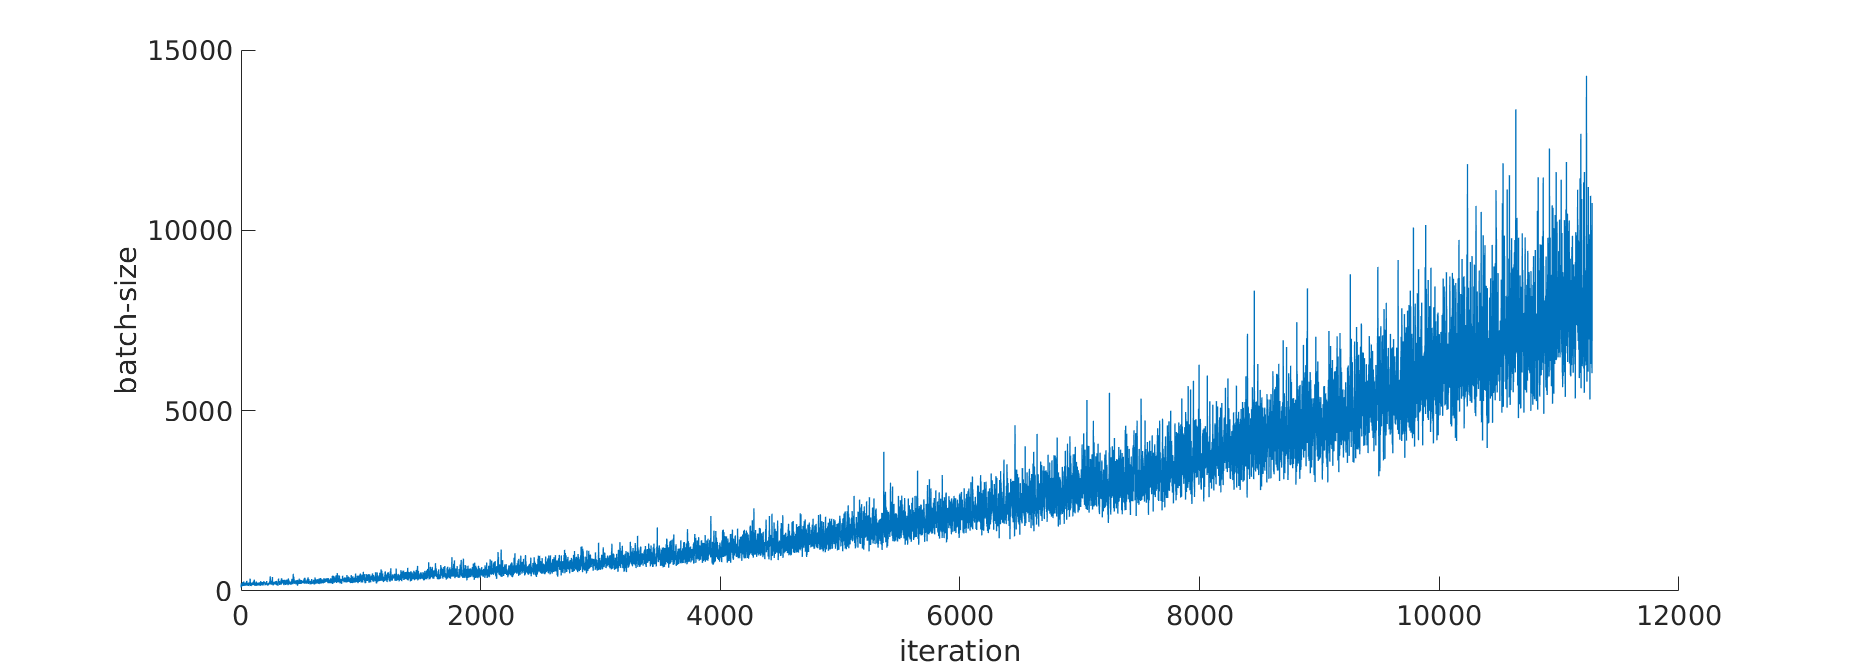
\includegraphics[width = 0.7\linewidth]{Images/batchsize_bern_emp.png}
	\label{fig:7}
	}
\end{adjustbox}
\caption[Adaptive batch size over learning iterations in the one-dimensional LQG task for different concentration bounds.]{Adaptive batch size over learning iterations in the one-dimensional \ac{LQG} task for different concentration bounds. In all the cases, the G(PO)MDP gradient estimator and $\delta=0.95$ were used.}
\label{fig:8}
\end{figure}


As expected, the batch size increases as the optimal parameter is approached, since positive improvements require more and more accuracy. The trend is evidently superlinear, with the exception of Hoeffding's bound with the theoretical range bound, which however selects very high batch sizes from the beginning. 

In all the experiments, the step size $\alpha$ is of the order of $10^{-6}$ and does not change significantly over learning iterations.


\section{Multi-dimensional LQG}\label{sec:lqg2d}
The one-dimensional \ac{LQG} problem was a good benchmark to compare the performance of different concentration bounds, but does not capture at all the coordinate descent aspect of our algorithm. Luckily, \ac{LQG} can easily be generalized to any number of dimensions $m$.

Following the approach of \cite{Pirotta:2015:MRL:2888116.2888124}, we define multi-dimensional \ac{LQG} as an \ac{MDP} with transition model:
\[
	\boldsymbol{s}_{t+1} \sim \mathcal{N}(\boldsymbol{s}_t+\boldsymbol{a}_t,C_0),
\] 

reward function:
\[
	r_t=-0.5(\boldsymbol{s}_t^TQ\boldsymbol{s}_t + \boldsymbol{a}_t^TR\boldsymbol{a}_t),
\]
and Gaussian policy:
\[
	\boldsymbol{a_t} \sim \mathcal{N}(\vtheta \cdot \boldsymbol{s}_t,C),
\]
where both $\boldsymbol{s}$ and $\boldsymbol{a}$ are vectors of size $m$, $C_0$ and $C$ are covariance matrices, $Q$ is a semidefinite matrix and $R$ is a symmetric positive definite matrix. All the matrices are $m\times m$. Note that also $\theta$ is an $m \times m$ matrix:
\[
\vtheta = \begin{bmatrix}
\theta_{11} & \theta_{12} \\
\theta_{21} & \theta_{22}
\end{bmatrix}
\]
Similarly to the one-dimensional case, we set $C_0=\boldsymbol{0}$ without loss of generality. Matrices $Q$ and $R$ can be used to define different objectives.

\subsection{Independent action in two dimensions}
By setting $Q$ and $R$ to the identity matrix and using a diagonal covariance $C$, the result are two simultaneous, independent one-dimensional \ac{LQG} problems. Although this fact is intuitive, it may not be trivial for a learning algorithm to exploit it. In particular, we consider the two dimensional case ($m=2$), with covariance matrix:
\[
	C = 
	\begin{bmatrix}
	\sigma_1 & 0 		\\
	0		 & \sigma_2
	\end{bmatrix}.
\]
In particular, in our experiments, we use $\sigma_1 = \sigma_2 = 1$ and $\gamma = 0.95$. With these parameters, the optimal parameter matrix is (approximately):
\[
	\vtheta^* \simeq 
	\begin{bmatrix}
	-0.588 & 0 		\\
	0		 & -0.588
	\end{bmatrix},
\]
with corresponding expected performance $J_\mu(\vtheta^*) \simeq -422.616$. The fact that $\vtheta$ is diagonal is due precisely to the independence of the two one-dimensional \ac{LQG} tasks.

We test our adaptive algorithm on this task. We use the G(PO)MDP gradient estimator with optimal baseline, Bernstein's bound with empirical range and $\delta=0.95$.
Figure \ref{fig:10} shows the evolution of the batch size over the learning process in the adaptive case.

\begin{figure}[h!]
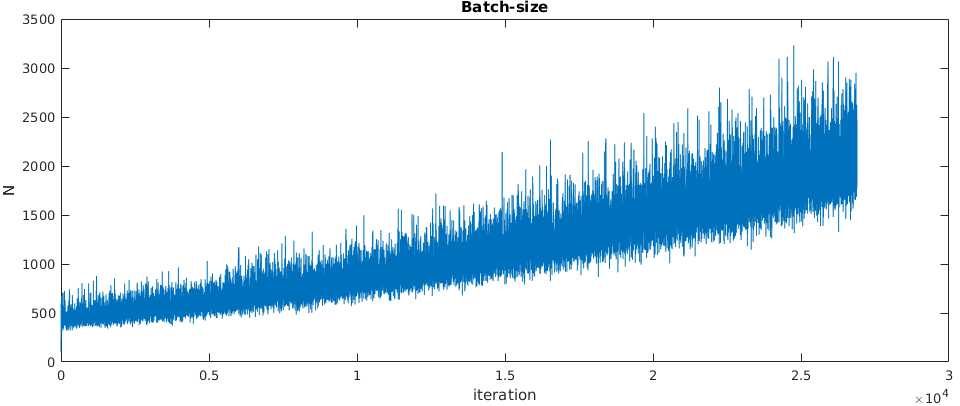
\includegraphics[width = 1.4\textwidth,left]{Images/lqg2d_batchsize.png}
\caption[Adaptive batch size over learning iterations in the two-dimensional LQG task.]{Adaptive batch size over learning iterations for the two-dimensional \ac{LQG} task. G(PO)MDP gradient estimator with optimal baseline, Bernstein's bound with empirical range and $\delta=0.95$ were used.}
\label{fig:10}
\end{figure}

The adaptive batch size goes from $N \simeq 500$ in the first learning iterations, to $N\simeq2500$ in the end. The step size takes values of the order of $1e-6$ for the whole process.
We compare the performance of our algorithm with the one of vanilla policy gradient with fixed step size and batch size. Since we want to focus our analysis to the effects of the batch size, we use G(PO)MDP with optimal baseline and $\alpha=1e-6$. We run two simulations, one with $N=1000$ and one with $N=100$. Figure \ref{fig:11} compares expected performance over learning iterations, while table \ref{tab:3} reports average performance $\overline{\Upsilon}$ and improvement ratio for the three cases.

\begin{figure}[h!]
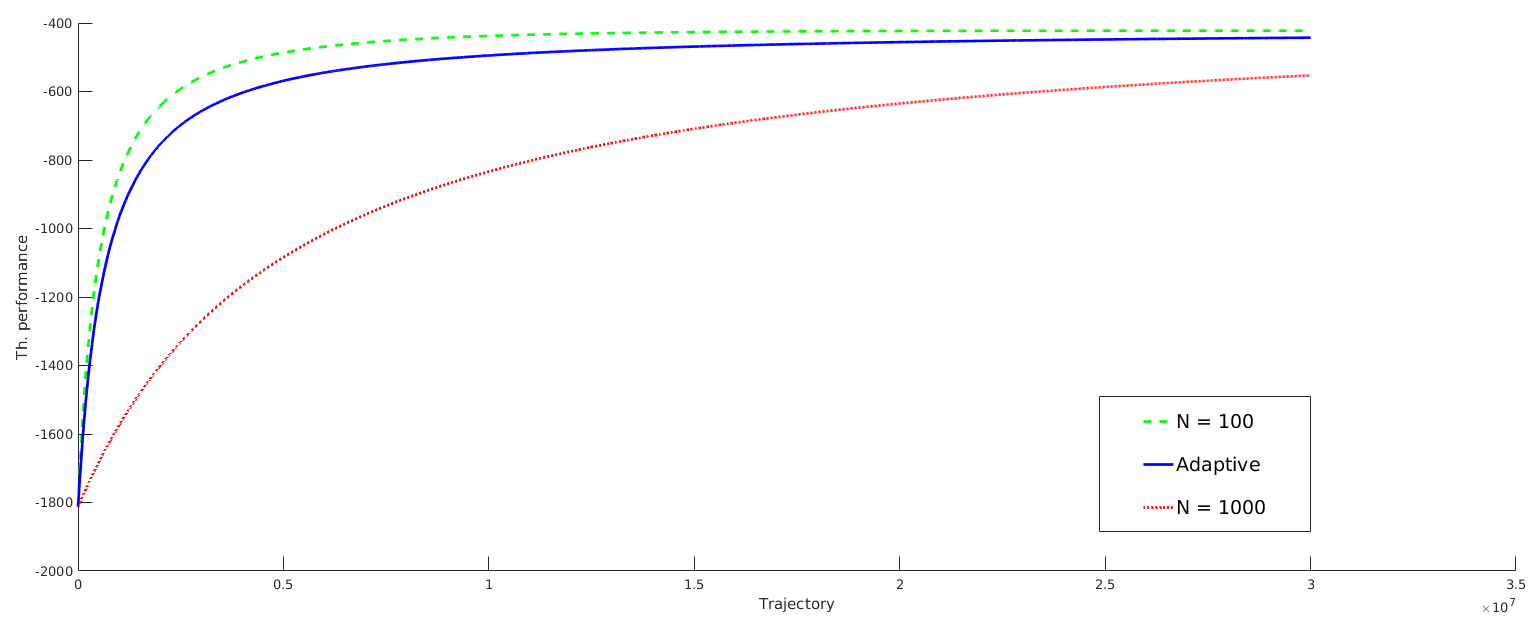
\includegraphics[width = 1.4\textwidth,left]{Images/lqg2d.png}
\caption[Expected performance over learning iterations in the two-dimensional LQG task.]{Expected performance over learning iterations in the two-dimensional \ac{LQG} task. The adaptive algorithm with Bernstein's bound and $\delta=0.95$ is compared with vanilla policy gradient with fixed $N=100,1000$ and $\alpha=1e-6$.}
\label{fig:11}
\end{figure}

\begin{table}[h!]
\caption[Average performance and improvement ratio for different simulations on the two-dimensional LQG task.]{Average performance and improvement ratio for different simulations on the two-dimensional \ac{LQG} task, using the G(PO)MDP gradient estimator with optimal baseline. The adaptive batch size is computed using Bernstein's bound with empirical range and $\delta=0.95$. The fixed batch sizes are used in conjunction with $\alpha=1e-6$.}
\label{tab:3}
\centering
\begin{adjustbox}{center}
\begin{tabular}{@{}lcc@{}} 
\toprule
N & $\overline{\Upsilon}$ & Improvement Ratio \\
\midrule
Adaptive & -20.50 & 100\% \\
1000 & -20.50 & 100\% \\
100 & -19.77 & 0.89\% \\
\bottomrule
\end{tabular}
\end{adjustbox}
\end{table}

Results show how a large, fixed batch size can badly affect the convergence rate. Our algorithm is able to outperform the $N=1000$ case by safely employing smaller batch sizes at the beginning of the learning process, turning to larger ones only when it is necessary.
For this task, a small batch size, such as $N=100$, yields a better average performance than our algorithm, but it introduces oscillation, witnessed by a less-than-one improvement ratio.
These results show how an adaptive batch size, such as the one employed by our algorithm, is able to guarantee monotonic improvement without needlessly sacrificing convergence speed.
\paragraph{}
Another interesting difference between our method and vanilla policy gradient is in the shape of the learned policy parameter $\theta$. In any stochastic policy gradient methods, the gradient components relative to $\theta_{12}$ and $\theta_{21}$ are small if compared to the other two, but not zero. This is due to noise and the result is that, even by starting from $\theta = \underline{0}$, the learned parameter will not be a diagonal matrix like the optimal one. On the contrary, a coordinate descent method like ours will never choose to update $\theta_{12}$ or $\theta_{21}$, because the gradient components associated to $\theta_{11}$ and $\theta_{22}$ are much larger. Starting from $\theta = \underline{0}$, a diagonal matrix is obtained.
Although this does not affect performance significantly, it shows how our algorithm is able avoid useless changes in the current policy, which are potential causes of oscillation. To support this analysis with real data, Table \ref{tab:4} shows the final value of $\vtheta$ for the usual three simulations.

\begin{table}[h!]\label{tab:4}
\caption[Final value of the policy parameter $\vtheta$ for different simulations on the two-dimensional LQG task.]{Final value of the policy parameter $\vtheta$,after a total of 30 million trajectories, for different simulations on the two-dimensional \ac{LQG} task, using the G(PO)MDP gradient estimator with optimal baseline. The adaptive batch size is computed using Bernstein's bound with empirical range and $\delta=0.95$. The fixed batch sizes are used in conjunction with $\alpha=1e-6$.}
\centering
\begin{adjustbox}{center}
\begin{tabular}{@{}ll@{}} 
\toprule
N & $\vtheta$ \\
\midrule
Adaptive & $\begin{bmatrix}
	-0.403 & 0 		\\
	0		 & -0.403
	\end{bmatrix}$\\
100 & $\begin{bmatrix}
	-0.6 & -1e-4 		\\
	1e-4		 & -0.6
	\end{bmatrix}$\\
1000 & $\begin{bmatrix}
	-0.21 & -1.7e-5 		\\
	-3.3e-5		 & -0.21
	\end{bmatrix}$\\
\bottomrule
\end{tabular}
\end{adjustbox}
\end{table}